\documentclass[a4paper, 12pt]{article}

\usepackage[utf8]{inputenc}
\usepackage[english]{babel}
\usepackage{amsmath}
\usepackage{amsfonts}
\usepackage{amssymb}
\usepackage{microtype}
\usepackage{enumitem}
\usepackage{listings}
\usepackage{graphicx}
\usepackage{subfig}
\usepackage{parskip}
\usepackage{authblk}

\begin{document}

\title{\Huge{\textbf{Elliptic Curves:}\\ Number Theory\\ and Cryptography}}
\author{Kethari Narasimha Vardhan\\ Tata Sai Manoj \\ Velagala Krishna Sai Deepak Reddy}
\affil{Group Project}
\date{February 12, 2022}

\maketitle
\pagenumbering{arabic}


\section{Chapter 1}
\section*{Introduction}
\subsection{Pyramid of Cannonballs}
Let us take a scenario where we put 1 ball at the first layer, 4 balls at the second layer, 9 balls at the third layer and so on {\dotso}Now, is it possible to arrange a total of n balls in a similar pattern such that all these balls can be fitted into a square array?\par
Mathematically, 
\begin{center}
Sum of all the balls would be; \par$1+2^2+3^2+\dotso+n^2 = \cfrac{(n)(n+1)(2n+1)}{6}$\par
The above expression should be a perfect square.\par
$\Rightarrow y^2 = \cfrac{(n)(n+1)(2n+1)}{6}$
\end{center}
An equation of the above form is called an \textbf{Elliptic Curve}.
\subsection{Elliptic Curve}
In mathematics, an elliptic curve is an equation of genus-1 surface. Genus, to simply put in, is the number of ``holes" of a surface. Elliptic Curves are important in Number Theory aspects and find applications in Elliptic Curve Cryptography (ECC). These are used in encryptions, digital signatures, pseudo-random number generators and few other areas.\par
The general equation of an elliptic curve $E$ is:
\begin{center}
$y^2 = x^3+Ax+B,$
\end{center}
where $A$ and $B$ are constants.
\subsection*{Examples:}
\begin{enumerate}[label=(\roman*)]
	\item Pyramid of Cannonballs 
	\begin{itemize}
		\item The above mentioned example when put in mathematical terms, yeilds an Elliptic Curve $y^2 = \cfrac{(x)(x+1)(2x+1)}{6}$
	\end{itemize}
	\item A right angle triangle with area $5$ and having rational side lengths.
	\begin{itemize}
		\item Let $a, b, c$ be the sides of the right angle triangle. Then, we need $a^2 + b^2 = c^2$, such that the area of the triangle is 5 and all the three sides must be rational.
		\item Now, let us assume $x = (c/2)^2$, \newline So we have $x-5 = ((a-b)/2)^2,$ \newline and $x+5 = ((a+b)/2)^2.$
		\item We are looking for a rational number $x$, such that $x-5,\; x,\: x+5$ are simultaneously squares of rational numbers. So the product, $(x-5)(x)(x+5)$ should also be a perfect square.
		\begin{center} $\Rightarrow y^2 = x^3 - 25x$ \end{center}
		This equation is an elliptic curve.
		\item The above equation has infinitely many solutions.
	\end{itemize}
	A more general case is, a right angle triangle with area $N$ and having rational sides. The elliptic curve in such scenario would be;
	\begin{center} $y^2 = (x-N)(x)(x+N)$ \par
	$\Rightarrow y^2 = x^3 - N^2x$
	\end{center}
	The integer $N$ which can occur as an area of a right angle triangle can be seen as \textit{Congruent Number Problem}. Tunnel's theorem relates this to the number of integral solutions of a few fairly simple \textit{Diophantine Equations}. But Tunnel Theorem gives only partial resolution to the Congruent Number Problem. \par
	\textbf{Diophantine Equation:} Finding all the right angle triangles with integer solutions is equivalent to solving the Diophantine equation $a^2+b^2=c^2$ \par
	\textbf{Conjecture:} Let $n$ be an odd, squarefree, positive integer. Then $n$ can be expressed as the area of a right angle triangle if and only if, the number of integer solutions of 
	\begin{center}$4x^2+y^2+8z^2=n$ \end{center} when $z$ is even is equal to number of solutions when $z$ is odd.
\end{enumerate}
\begin{figure}
    \centering
    \subfloat[\centering $y^2 = \frac{(x)(x+1)(2x+1)}{6}$]{{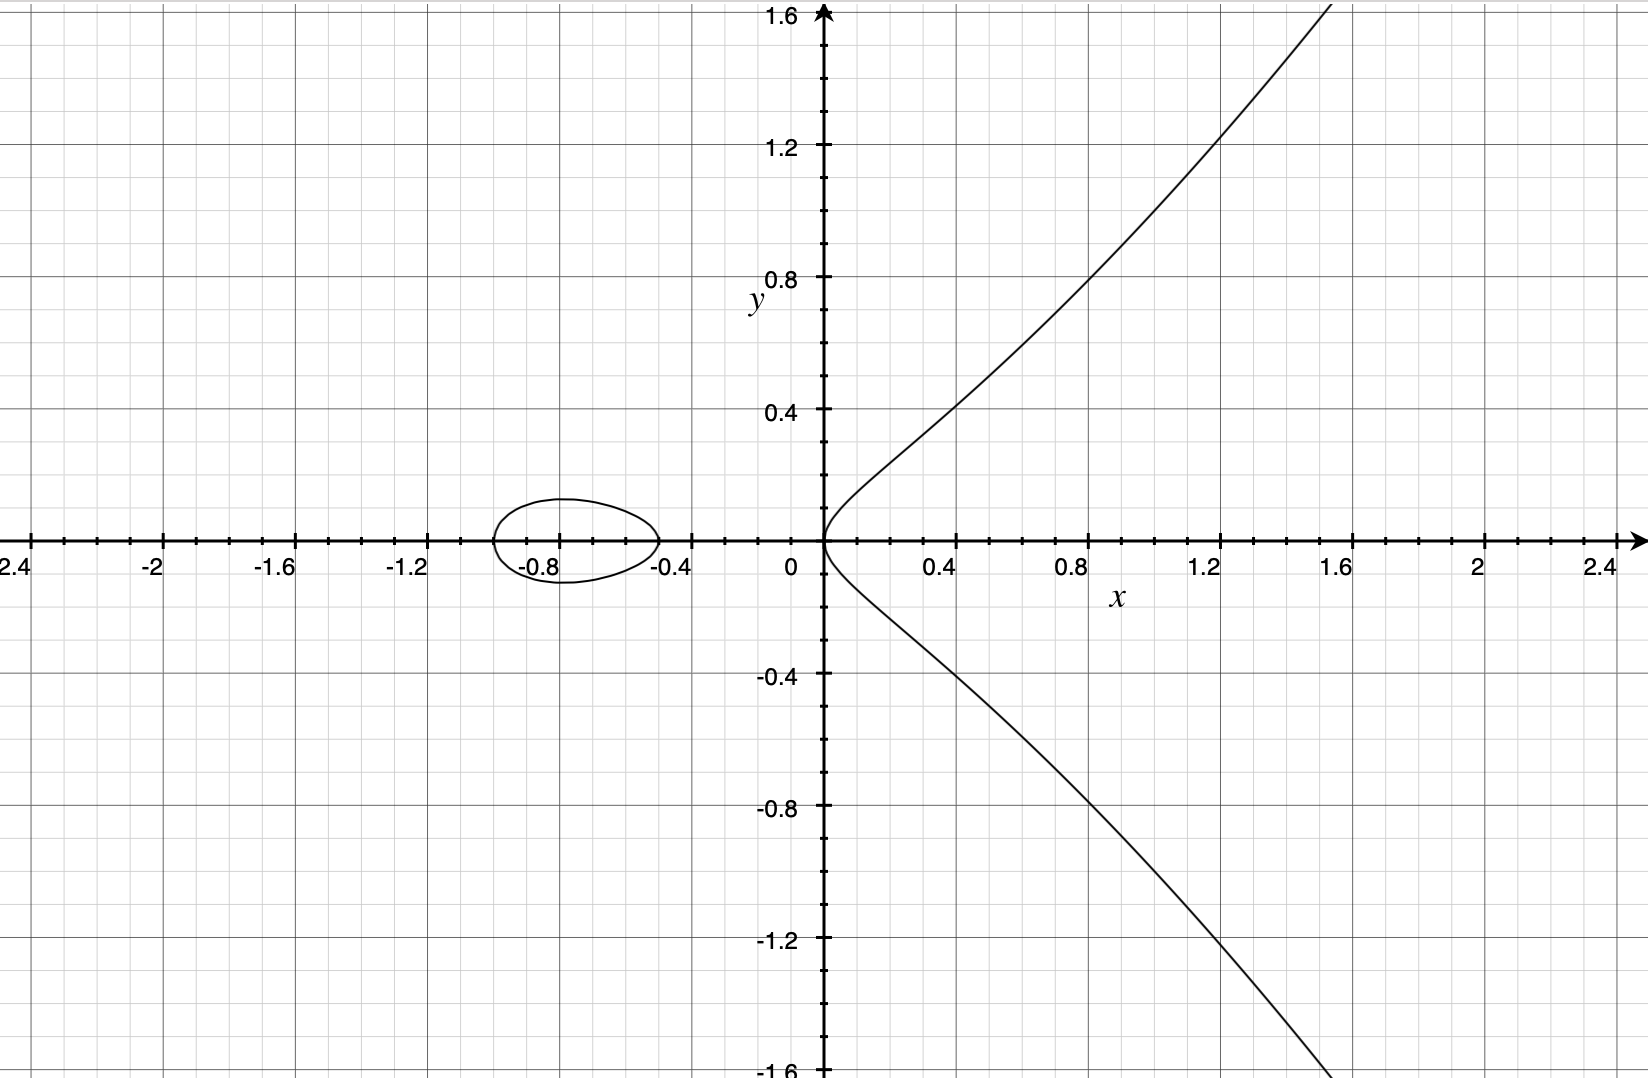
\includegraphics[width=6cm]{1} }}
    \qquad
    \subfloat[\centering $y^2 = x^3 - 25x$]{{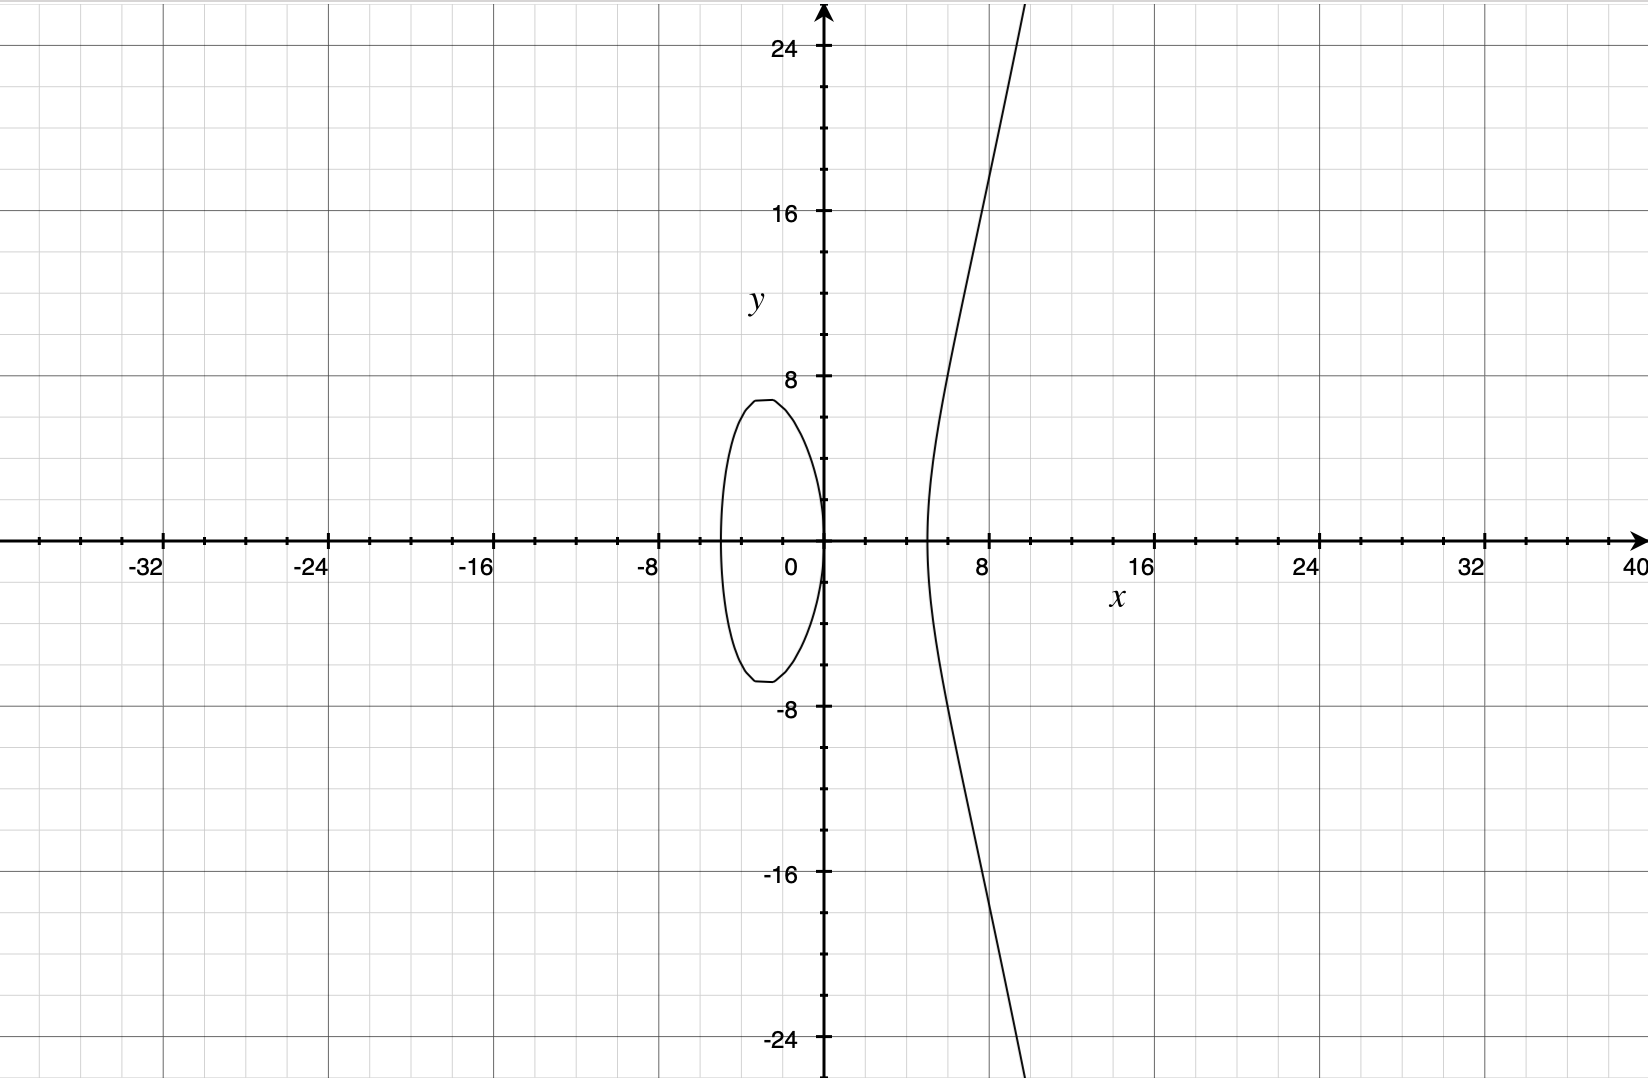
\includegraphics[width=6cm]{2}}}
    \caption{Elliptic Curves of (i) and (ii)}
    \label{fig:example}
\end{figure}
\section{Chapter 2}
\section*{The Basic Theory}
\subsection{Weierstrass Equation}
As seen earlier, an elliptic curve $E$ is a graph with general equation
\begin{center}$y^2=x^3+Ax+B,$\end{center}
where $A$ and $B$ are constants. The above equation is known as \textbf{Weierstrass Equation} for an elliptic curve. It is important to note as in what set $A, B, x,$ and $y$ belong to. Generally, these are the elements taken from a field.\par
\textbf{Field:} In mathematics, a field is a set on which basic mathematical operations are defined and behave as corresponding operations on rational and real numbers do. Such as addition, multiplication, subtraction, and division. A field is an \textit{algebraic structure} that is widely used in algebra, number theory.\par
Few examples of fields are the field of rational numbers, the field of real numbers, the field of complex numbers. Finite Fields (fields with finitely many elements) are mostly used in cryptographic protocols.\par
\textbf{Algebraic Structure:} An algebraic structure consists of a nonempty set $A$, a collection of operations on $A$, in general binary operations $*$, and finite set of identities that these operations must satisfy.\par
A group is an example of examples of algebraic structures. The various types of algebraic structures are:
\begin{itemize}
	\item Semigroup
	\item Monoid
	\item Group
	\item Abelian Group
\end{itemize}
Let us take an algebraic structure $(\mathbb{Z},+)$. This is also an example of a group, that satisfies all the conditions of a group, \textit{i.e.,} Closure, Associative, Identity Element, and Inverse Element.
\begin{center}
Here, set $A$ is set of all integers $\mathbb{Z}$, and\par
the binary operation $*$ is addition $(+)$
\end{center}\par
Now, let us take $K$, that is a field with $A,B\in K$, then we say that the elliptic curve \textbf{$E$ is defined over $K$}. If we want to consider points with coordinates in a field $L$ which is a superset of $K$ $(L\supseteq K )$, then $E(L)$ is defined as
\begin{center}
$E(L) = \{\infty\}\: \cup\: \{(x,y)\in L \times L\:|\:y^2=x^3+Ax+B\}.$
\end{center}
This set $E(L)$ always contains the point $\infty$ in it.\par
If the roots of the cubic equation are $r_1,r_2,r_3$, then it can be proved that the discriminant of the cubic equation is
\begin{center}
$((r_1-r_2)(r_2-r_3)(r_3-r_1))^2=-(4A^3+27B^2).$
\end{center}
Therefore, we keep the roots of the cubic to be distinct. However, there are cases where the roots are not distinct. Thus, a more generalized equations are of the form,
\begin{center}
$y^2+a_1xy+a_3y=x^3+a_2x^2+a_4x+a_6$,
\end{center}
where $a_1,a_2,\dotso,a_6$ are constants. The above equation is called \textbf{Generalized Weierstrass Equation}. These equations are useful when the fields have characteristic 2 or 3.\par
\textbf{Characteristic:} Denoted by \textit{char(.)}, is defined by the smallest number of times the multiplicative identiy is to be used to get the additive identity of a ring/group. If the sum never reaches the additive identity, we say that the characteristic of the ring/group is zero.\par
The characteristic of any field $F$ is either 0 or a prime number $p$.
\subsection{The Group Law}
Let $E$ be an elliptic curve defined as $y^2=x^3+Ax+B$. Let us take two distinct points on the curve E, $P_1=(x_1,y_1)$ and $P_2=(x_2,y_2)$ with $P_1,P_2 \neq \infty$. Let $L$ be a line through $P_1$ and $P_2$, and this line $L$ intersects the curve $E$ at $P_3'$. Now, take a reflection of $P_3'$ across the $x-$axis to get a new point $P_3=(x_3,y_3).$\par
Then, we define $P_1+P_2=P_3=(x_3,y_3)$ as:
\begin{itemize}
	\item If $x_1\neq x_2$, then\newline 
	$x_3=m^2-x_1-x_2,$ \qquad $y_3=m(x_1-x_3)-y_1,$\qquad where $m=\cfrac{y_2-y_1}{x_2-x_1}$
	\item If $x_1=x_2$ but $y_1\neq y_2$, then $P_1+P_2=\infty$\par
	Since the line $L$ joining $P_1$ and $P_2$ would be a vertical line parallel to the $y-$axis. Thus, the line $L$ doesn't intersect the curve $E$ for any $P_3$.
	\item If $P_1=P_2$ and $y_1\neq 0$, then\newline
	$x_3=m^2-2x_1,$ \qquad $y_3=m(x_1-x_3)-y_1,$\qquad where $m=\cfrac{3x_1^2+A}{2y_1}$
	\item If $P_1=P_2$ and $y_1=0$, then $P_1+P_2=\infty$\par
	Since the line $L$ joining $P_1$ and $P_2$ would be a vertical line and a tangent line to the curve $E$.
\end{itemize}
\subsubsection{Theorem}
The points on the curve $E$ form an algebraic structure $i.e.,$ they form a group. Moreover, they form an abelian group with $\infty$ as it's identity element.\par
\begin{itemize}
	\item \textit{Commutativity:} $P_1+P_2=P_2+P_1,\:\:\forall\: P_1, P_2 \in E$.
	\item \textit{Existence of Identity:} $P+\infty=P,\:\:\forall\: P \in E$.
	\item \textit{Existence of Inverse:} Given $P$ $\in$ $E,\: \exists\: P' \in E$ such that $P+P'=\infty$. The point $P'$ is denoted by $-P$.
	\item \textit{Associativity:} $(P_1+P_2)+P_3=P_1+(P_2+P_3),\:\:\forall \:P_1,P_2,P_3 \in E$.
\end{itemize}
$\square$\newline
According to the 2.2.1 Theorem, it is said that the points on the elliptic curve $E$ form an abelian group. 
\begin{enumerate}
	\item An elliptic curve over a finite field has only finitely many points with coordinated in that finite field. Therefore, we obtaion finite abelian group in this case.
	\item Let $E$ be an elliptic curve defined over $\mathbb{Q},$ then $E(\mathbb{Q})$ is a finite abelian group.\end{enumerate}
If $P$ is a point on the curve $E$, and let $k$ be any positive integer. Then $kP$ denotes, $P+P+\dotso +P\: (k$ times). For large values of $k$, repeatedly adding $P$ to itself is computationally heavy task. The computation becomes much faster when \textit{succcessive doubling} method is used. \newline Eg. Compute $19P$;
\begin{center}
$2P,\quad 4P=2P+2P,\quad 8P=4P+4P,\quad 16P=8P+8P,$ \newline thus $\Rightarrow19P=16P+2P+P$.
\end{center}
\subsubsection{Integer Times a Point}
\textbf{NOTE:} If we are working over a large finite field and are given points $P$ and $kP$, it is computationally difficult to determine the value of $k$. This is known as the \textbf{Discrete Logarithm Problem} for elliptic curves and is the basis for the cryptographic applications.\par
Let us take $k$ to be any positive integer and let $P$ be a point on the elliptic curve $E$. Then, to compute $kP$:\par
\begin{enumerate}
	\item Start with $a=k, B=\infty, C=P$.
	\item If $a$ is even, then $a=a/2$, and $C=2C$.
	\item If $a$ is odd, then $a=a-1$, and $B=B+C$.
	\item If $a \neq 0$, repeat from step 2.
	\item Output $B$.
\end{enumerate}
\lstinputlisting{code2.py}\par
\subsection{Projective Space and the Point at Infinity}
Projective Spaces allow us to interpret the point at infinity on an elliptic curve. Also, it says that parallel lines meet at infinity. In terms of Linear Algebra, a projective space of dimension $n$ is defined as the set of the \textbf{vector line} (a vector subspace of dimension 1) in vector space $V$ of $n+1$ dimension.
A position vector describes the straight-line travel between a starting point (usually the origin) and the location of a second point on a coordinate plane is called a vector line.\par
Let $K$ be a field. A 2-D \textbf{projective space $P_K^2$} over $K$ is given by the equivalence classes of triples $(x,y,z)$ with $x,y,z \in K$. Two triples $(x_1,y_1,z_1)$ and $(x_2,y_2,z_2)$ are said to be \textbf{equivalent} if there exists a nonzero element $\lambda \in K$, such that
\begin{center}
$(x_1,y_1,z_1) = (\lambda x_2,\lambda y_2, \lambda z_2)$
\end{center}
We write such a relation as $(x_1,y_1,z_1) \sim (x_2,y_2,z_2)$. This class of triples depends on the ratios of $x$ to $y$ to $z$. Thus, the equivalence class is denoted by $(x:y:z)$.\par
We can write $(x:y:z)$ as $(x/z:y/z:1)$ which represent ``finite'' points in \textbf{$P_K^2$}. And if $z=0$, then the ratio becomes $(x:y:0)$ which are called the \textbf{``points at infinity''} in \textbf{$P_K^2$}. \par
The two-dimensional \textbf{affine plane} over $K$ is denoted as:
\begin{center} $\mathbb{A}_K^2 = \{(x,y)\in K$ x $K\}$\end{center}
\textbf{Affine Plane:} In geometry, an affine plane is a system of points and lines that satisfy the below conditions. Note that in an affine plane, two lines are called \textit{parallel} if they are equal disjoint. 
\begin{itemize}
	\item Any two distinct points lie on a unique line.
	\item Each line has at least two points.
	\item Given a point and a line, there is a unique line which contains the point and is parallel to the line (From the Note point).
	\item There exist three non-collinear points.
\end{itemize}
Parallelism, the state of being parallel is an equivalence relation on the lines of an affine plane. \textit{Euclidean Plane} is a familiar affine plane. There are also many finite and infinite affine planes. \par
\textbf{Finite Affine Plane:} If the number of points in an affine plane is finite, then if one line contains $n$ points, then:
\begin{itemize}
	\item each line contains $n$ points.
	\item each point is contained in $n+1$ lines.
	\item there are $n^2$ points in all.
	\item there is a total of $n^2 + n$ lines.
\end{itemize}
Here, the number $n$ is called the \textit{order} of the affine plane. All knows finite affine planes have order as either a prime number or prime power integer.\par
Now, let us take an inclusion,
\begin{center} $\mathit{A}_K^2\hookrightarrow \mathit{P}_K^2$ \end{center} given by
\begin{center} $(x,y) \mapsto (x:y:1)$ \end{center}
Thus, the affine plane is identified with the finite points in $\mathbb{P}_K^2$. 
Example:\par
If $f(x,y)$ is a polynomial in $x$ and $y$, then we can make it homogeneous by inserting appropriate powers of $z$. Let us take A$f(x,y)=y^2-x^3-Ax-B$, then we obtain the homogeneous polynomial $F(x,y,z)=y^2z-x^3-Axz^2-bz^3$. If $F$ is homogeneous of degree $n$, then:
\begin{center} $F(x,y,z)=z^nf(\cfrac{x}{z},\cfrac{y}{z})$ and $f(x,y)=F(x,y,1)$\end{center}
Now, let us take an Elliptic Curve $E$ defined as $y^2=x^3+Ax+B$. The homogeneous form of this curve $E$ would be $y^2z=x^3+Axz^2+Bz^3$. The points $(x,y)$ on the original curve correspond to the points $(x:y:1)$ in this new projective version. To see what points on $E$ lie at infinity, set $z=0$ and obtain $0=x^3$. Thus, $x=0$, and $y$ can be any nonzero number (NOTE: $(0:0:0)$ is not allowed). Rescaling $y$ as, $(0:y:0) = (0:1:0)$ is the point at infinity on $E$. Moreover, since $(0:1:0) = (0:-1:0)$, the ``top'' and the ``bottom'' of the $y-$axis are the same.\par
There are situations where using projective coordinates sppeds up the computational aspects on elliptic curves. 
\subsection {Proof of Associativity}
Associativity of addition of points on an elliptic curves. Two most important theorems that are not about elliptic curves but are quite fascinating here are Pappus and Pascal.\par
\subsubsection{Lemma:}  
Let $G(u,v)$ be a nonzero homogeneous polynomial and let $(u_0:v_0)\in \mathbb{P}_K^1$. Then there exists an integer $k \geq 0$ and a polynomial $H(u,v)$ with $H(u_0,v_0) \neq 0$ such that
\begin{center} $G(u,v)=(v_0u-u_0v)^kH(u,v)$\end{center}\par
$\square$\newline
Let $f(x,y)=0$ be a polynomial describing a curve $C$ in the affine plane and let
\begin{center} $x=a_1t+b_1,\: y=a_2t+b_2$ \end{center}
be a line $L$ written in terms of the parameter $t$. And let,
\begin{center} $\tilde{f}(t) = f(a_1t+b_1,a_2t+b_2).$ \end{center}
The line $L$ intersects the curve $C$ at suppose $t=t_0$ if $\tilde{f}(t_0)=0$. If $(t-t_0)^2$ divides $\tilde{f}(t)$, the $L$ is a tangent to $C$. To keep it more general, we say that $L$ intersects $C$ to order $n$ at the point $(x,y)$ corresponding to $t=t_0$ if $(t-t_0)^n$ is the highest power of $(t-t_0)$ that divides $\tilde{f}(t)$.\par
The homogeneous polynomial of the above can be described as 
\begin{center}
$\tilde{F}(u,v) = F(a_1u+b_1v,a_2u+b_2v,a_3u+b_3v)$
\end{center}
Here, we say that $L$ intersects $C$ to order $n$ at the point $P = (x_0:y_0:z_0)$ corresponding to $(u:v) = (u_0:v_0)$ if $(v_0u-u_0v)^n$ is the highest power of $(v_0u-u_0v)$ dividing $\tilde{F}(u,v)$. We denote this by
\begin{center} $ord_{L,P}(F) = n$ \end{center}
If $\tilde{F}$ is identically 0, then we let $ord_{L,P}(F) = \infty$. The major advantage of the homogeneous formulation is that it allows us to treat the points at infiinty along with the finite points in a uniform manner.\par
\subsubsection{Lemma: }
Let $L_1$ and $L_2$ be lines intersecting in a point $P$, and, for $i = 1, 2$, let $L_i(x,y,z)$ be a linear polynomial defining $L_i$. Then $ord_{L_1,P}(L_2) = 1$ unless $L_1(x,y,z) = \alpha L_2(x,y,z)$ for some constant $\alpha$, in which case $ord_{L_1,P}(L_2) = \infty$.
\subsubsection{Definition: }
A curve in $\mathbb{P}_K^2$ defined by $F(x,y,z) = 0$ is said to be \textbf{non-singular} at a point $P$ if at least one of the partial derivatives $F_x,F_y,F_z$ is nonzero at $P$.\par
Let us take an Elliptic Curve $F(x,y,z) = y^2z - x^3 - Axz^2  Bz^3 = 0$, and let us assume the characteristic of our field $K$ is not 2 or 3. Now, we have
\begin{center}
$F_x = -3x^2 - Az^2$\par
$F_y = 2yz$\par
$F_z = y^2 - 2Axz - 3Bz^2$
\end{center}
Suppose $P = (x:y:z)$ is a singular point. It can be easily shown that for any values of $x, y, z$, there occurs a contradiction for Elliptic Curves. Therefore, \textbf{an elliptic curve has no singular points}. \newline
NOTE: This is true even if we consider points with coordinates in $\overline{K}$ ($=$ algebraic closure of $K$). In general, by a \textbf{non-singular curve}, we mean a curve with no singular points in $\overline{K}$.
$\square$\newline
If $P$ is a nonsingular point of a curve $F(x,y,z)=0$, then the tangent line at $P$ is
\begin{center}
$F_x(P)x + F_y(P)y + F_z(P)z = 0$
\end{center}
The above equation leads us to the fact that $\infty + \infty = \infty$ on an elliptic curve.
\subsubsection{Lemma: }
Let $F(x,y,z)=0$ define a curve $C$. If $P$ is a nonsingular point of $C$, then there is exactly one line in $\mathbb{P}_K^2$ that intersects $C$ to order at least 2, and it is the tangent to $C$ at $P$.\par
Didn't understand this proof.
$\square$
\subsubsection{Theorem: }
Let $C(x,y,z)$ be a homogeneous cubic polynomial, and let $C$ in $\mathbb{P}_K^2$ described by $C(x,y,z)=0$. Let $l_1,l_2,l_3$ and $m_1,m_2,m_3$ be lines in $\mathbb{P}_K^2$ such that $l_i \neq m_j$ for all $i,j$. Let $P_{ij}$ be the point of intersection of $l_i$ and $m_j$. Suppose $P_{ij}$ is a nonsingular point on the curve $C$ for all $(i,j) \neq (3,3)$.\newline
In Addition, we require that if, for some $i$, there are $k \geq 2$ of the points $P_{i1},P_{i2},P_{i3}$ equal to the same point, then $l_i$ intersects $C$ to order at least $k$ at this point. Also, if, for some $j$, there are $k \geq 2$ of the points $P_{j1},P_{j2},P_{j3}$ equal to the same point, then $m_j$ intersects $C$ to order at least $k$ at this point. Then $P_{33}$ also lies on the curve $C$.\par
\textbf{Proof: } Express $l_1$ in the parametric form. Then $C(x,y,z)$ becomes $\tilde{C}(u,v)$. The line $l_1$ passes through $P_{11},P_{12},P_{13}$. Let $(u_1:v_1),(u_2:v_2),(u_3:v_3)$ be the parameters on $l_1$ for these points. Since these points lie on $C$, we have $\tilde{C}(u_i,v_i) = 0$ for $i=1,2,3$.\par
Let $m_j$ have equation $m_j(x,y,z)=a_jx+b_jy+c_jz=0$. Substituting the parameterization for $l_1$ yields $\tilde{m}_j(u,v).$ Since $P_{ij}$ lies on $m_j$, we have $\tilde{m}_j(u_j,v_j)=0$ for $j=1,2,3$. \newpage Since $l_1 \neq m_j$ and since the zeros of $\tilde{m}_j$ yield the intersections of $l_1$ and $m_j$ , the function $\tilde{m}_j(u,v)$ vanishes only at $P_{1j}$, so the linear form $\tilde{m}_j$ is nonzero. Therefore, the product $\tilde{m}_1(u,v)\tilde{m}_2(u,v)\tilde{m}_3(u,v)$ is a nonzero cubic homogeneous polynomial. We need to relate this product to $\tilde{C}$.$\blacksquare$
\subsection{Other Equations for Elliptic Curves}
Generally, we are mainly dealing with Weierstrass Equation of Elliptic Curves. However, elliptic curves arise in various other guises.
\subsubsection{Legendre Equation}
This is a variant on the Weierstrass Equation. It's advantage is that it allows us to express all elliptic curves over an algebraically closed field (characteristic $\neq 2$) in terms of one parameter.\par
Let $K$ be a field of characteristic not 2 and let
\begin{center} $y^2 = x^3 + ax^2 + bx + c = (x - e_1)(x - e_2)(x - e_3)$ \end{center}
be an elliptic curve $E$ over $K$ with $e_1,e_2,e_3 \in K$. Let
\begin{center}
$x_1 = (e_2 - e_1)^{-1}(x - e_1),$  \:\: $y_1=(e_2-e_1)^{-3/2},$  \:\: $\lambda = \cfrac{e_3-e_1}{e_2 -e_1}.$
\end{center}
Then $\lambda \neq 0,1$ and,
\begin{center} $y_1^2 = x_1(x_1-1)(x_1-\lambda)$. \end{center}
This equation has three singular points, $\lambda = 0,1,\infty$.
\subsubsection{Cubic Equations}
Let us consider a cubic Fermat equation $x^3+y^3+z^3=0.$\newline
This equatoin has no rational solutions with $xyz \neq 0$ was a conjecture and represents a special case of Fermat's Last Theroem, which asssets that the sum of two nonzero $n$th powers of integers cannot be a nonzer $n$th power when $n\geq 3$. \par
It is possible to start with a cubic equation $C(x,y)=0$, over a field $K$ of characteristics not 2 or 3, that has a point with $x,y\in K$ and find an invertible change of variables that transforms the equation to Weierstrass form.
\subsubsection{Quartic Equations}
Sometimes, we might come across few curves defined by the equation of the form
\begin{center}
$v^2=au^4+bu^3+cu^2+du+e,$
\end{center}
with $a \neq 0$. If we have a point $(p,q)$ lying on the curve with $p,q\in K$, then the equation can be transformed into a Weierstrass Equatoin by an invertible change of variables that uses rational functions wiht coefficients in the field $K$.
\newline
NOTE: If we are going to transform a curve $C$ into Weierstrass form in such a way that all coefficients of the rational functions describing the transformation lie in $K$, then we need to start with a point on $C$ that has coordinates in $K$.\par
Suppose we have a curve defined by the above equation and suppose we have a point $(p, q)$ lying on the curve. By changing $u$ to $u + p$, we may assume $p = 0$, so the point has the form $(0, q)$.
\begin{center}
$(\cfrac{v}{u^2})^2=d(\cfrac{1}{u})^3 + c(\cfrac{1}{u})^2 + b(\cfrac{1}{u}) + a$.
\end{center}
This can be easily transformed into a Weierstrass Equation in $d/u$ and $dv/u^2$. \par
\textbf{Theorem:}\par
Let $K$ be a field of characteristic not 2. Consider the equation
\begin{center}
$v^2=au^4+bu^3+cu^2+du+q^2$
\end{center}
with $a,b,c,d,q \in K.$ Let,
\begin{center}
$x = \cfrac{2q(v+q) + du}{u^2},$  \:\: $y = \cfrac{4q^2(v+q)+2q(du+cu^2)-(d^2u^2/2q)}{u^3}$.
\end{center}
Now, define
\begin{center}
$a_1 = d/q, \:\: a_2=c-(d^2/4q^2), \:\: a_3=2qb, \:\: a_4=-4q^2a, \:\: a_6=a_2a_4$
\end{center}
Then,
\begin{center}
$y^2 + a_1xy + a_3y = x^3 + a_2x^2 + a_4x + a_6.$
\end{center}
The inverse transformation is 
\begin{center}
$u =\cfrac{2q(x+c) - (d^2/2q)}{y}, \:\: v = -q+\cfrac{u(ux-d)}{2q}.$
\end{center}
The point $(u,v) = (0,q)$ corresponds to the point $(x,y)=\infty$ and $(u,v)=(0,-q)$ corresponds to $(x,y)=(-a_2,a_1a_2-a_3)$.
\subsubsection{Intersection of Two Quadractic Surfaces}
The intersection of two quadractic surfaces in three-dimensional space, along with a point on this intersection, is usually an elliptic curve.
DOUBT HEREEEEEE\par
Let us consider pairs of equations of the form
\begin{center} $au^2+bv^2=3,\quad cu^2+dw^2=f,$ \end{center}
where $a,b,c,d,e,f$ are nonzero elements of a field $K$ of characteristic not 2. Each separeate equation may be regarded as a surface in $uvw$-space, and they intersect in a curve. 
Let's take $P=(u_0,v_0)$ be a point on $C$, where $C$ is a curve in the $uv$-plane. Let $L$ be the line through $P$ with slope $m$, 
\begin{center} $u=u_0+t,\quad v=v_0+t$. \end{center}
We want to find another point $(u,v)$ which is formed at the second intersection point of line $L$ and curve $C$. The new point $(u,v)$ can be given by,
\begin{center}
$u = u_0 - \cfrac{2au_0+2bv_0m}{a+bm^2}, \quad v = v_0 - \cfrac{2amu_0+2bv_0m^2}{a+bm^2}.$
\end{center}
To derive the above values of $u$ and $v$, we use the fact that $au_0^2+bv_0^2=e$.\par
We now want to intersect $C$, regarded as a ``cylinder'' in $uvw$-space, with the surface $cu^2+dw^2=f$. 
\begin{center} $dw^2 = f - c\left( u_0 - \cfrac{2au_0+2bv_0m}{a+bm^2}\right)^2$ \end{center}
This above equation can be changed to Weierstrass from. If $w_0=0$, then fourth degree polynomial becomes a cubic polynomial, so the equation just obtained is easily put into Weierstrass form. The procedure of changing ``square = degree four polynomial'' into Weierstrass form requires a point satisfying thie equation.\par Trying with an example, let us take 
\begin{center}$u^2+v^2=2,\quad u^2+4w^2=5.$\end{center}
First, we parameterize the solutions of $u^2+v^2=2$. Then, finding the values of $u, v$ in terms of slope $m$. \newline
Substituting the values of $u,v$ in $u^2+4w^2=5$, with a little bit of manipulation, the formulas then change this curve to generalized Weierstrass equation
\begin{center} $y^2-xy+2y=x^3+\cfrac{7}{4}x^2-4x-7.$\end{center}
\subsection{The j-invariant}
If we have 2 elliptic curves $E_1$ and $E_2$, we use the ``j-invarinat'' concept to check whether the 2 curves are isomorphic or not. \newline Let $E$ be the elliptic curve given by $y^2=x^3+Ax+B$, where $A, B$ are elements of a filed $K$ of characteristic not 2 or 3. Let us consider 
\begin{center} $x_1 = \mu^2x,\quad y_1=\mu^2 y, $ \end{center}
with $\mu \in {\bar{K}}^X$, then we obtain a new curve as
\begin{center} $y_1^2 = x_1^3+A_1x_1+B_1,$ \end{center}
with \begin{center} $A_1 = \mu^4A,\quad B_1=\mu^6B.$ \end{center}
Now, we define the \textbf{j-invariant} of $E$ to be
\begin{center} $j = j(E) = 1728\cfrac{4A^3}{4A^3+27B^2}.$ \end{center}
We also define $\Delta$ as $\Delta = 4A^3+27B^2$. Thus, the j-invariant would be
\begin{center} $j = j(E) = 1728\cfrac{4A^3}{\Delta}$ \end{center}
\subsubsection {Theorem}
Let $y_1^2 = x_1^3 + A_1x_1+B_1$ and $y_2^2 = x_2^3 + A_2x_2+B_2$ be two elliptic curves with $j-$invariant $j_1$ and $j_2$, respectively. If $j_1 = j_2$, then there exists $\mu \neq 0$ in $\bar{K}$ (= algebraic closure of $K$) such that
\begin{center} $A_2 = \mu^4A_1, \quad B_2=\mu^6B_1$ \end{center}
The transformation
\begin{center} $x_2=\mu^2x_1,\quad y_2=\mu^3y_1$ \end{center}
takes one equation to the other.\par
There are two special cases of $j$ that arise often:
\begin{itemize}
	\item $j=0:$ In this case, the elliptic curve $E$ has the form $y^2=x^3 +B.$
	\item $j=1728:$ In this case, the elliptic curve $E$ has the form $y^2=x^3+Ax.$
\end{itemize}

We say that the two elliptic curves $E_1$ and $E_2$ are isomorphic \textbf{iff} $j(E_1) = j(E_2)$
\par The j - invariant is a one dimensional space which parametrises Elliptic Curves. It is also called `Coarse Moduli Space' of Elliptic Curves.\par
The curves with $j=0$ and with $j=1728$ have automorphisms (bijective group homomorphisms from the curve to itself). Note that the $j-$invariant tells us when two curves are isomorphic over an algebraically closed field. However, if working with a nonalgebraically closed field $K$, then it is possible to have two curves with the same $j-$invariant that cannot be transformed into each other using rational functions with coefficients in $K$.\par
If two different elliptic curves defined over a field $K$ have the same $j-$invariant, then we say that the two curves are \textbf{twists} of each other. The $j$ is the $j-$invariant of
\begin{center} $y^2=x^3+\cfrac{3j}{1728-j}x + \cfrac{2j}{1728-j}$ \end{center}
when $j \neq 0,1728$.
\subsection{Elliptic Curves in Characteristic 2}
Most of the time, we used the Weiertrass equation rather than the generalized Weierstrass equation. That is, all the given formulas given do not apply when the field $K$ has characteristic 2. For the generalized Weierstrass equation for an elliptic curve $E$:
\begin{center} $y^2+a_1xy+a_3y=x^3+a_2x^2+a_4x+a_6$ \end{center}
If $a_1 \neq 0$, then the change of variables
\begin{center} $x=a_1^2x_1+(a_3/a_1),\quad y=a_1^3y_1+a_1^{-3}(a_1^2a_4+a_3^2)$ \end{center}
changes the equation to the form
\begin{center} $zy_1^2+x_1y_1=x_1^3+a_2'x_1^2+a_6'.$ \end{center}
This above curve is nonsingular if and only if $a_6' \neq 0$. The $j-$invariant in this case is defined to be $1/a_6'$.\par
If $a_1=0$, we let $x=x_1+a_2,y=y_2$ to obtain an equation of the form,
\begin{center} $y_1^2+a_3'y_1=x_1^3+a_4'x_1+a_6'.$ \end{center}
This above curve is nonsingular if and only if $a_3' \neq 0$. The $j-$invariant in this case is defined to be 0.\par
Making the equation homogeneous:
\begin{center} $y^2z+a_1xyz+a_3yz^2=x^3+a_2x^2z+a_4xz^2+a_6z^3.$ \end{center}
Now, set $z=0$, therefore $\infty = (0:1:0)$ is the only poiny at infinity on $E$. A line $L$ through $(x_0,y_0)$ and $\infty$ is a vertical line $x=x_0$. If $(x_0,y_0)$ lies on $E$, then the other point of intersection of $L$ and $E$ is $x_0,-a_1x_0-a_3-y_0)$. Now we can descrive the addition of points.
\subsection{Endomorphisms}
By an \textbf{endomorphism} of $E$, we mean a homomorphism $\alpha:E(\bar{K})\rightarrow E(\bar{K})$ that is given by rational functions. In other words, $\alpha(P_1+P_2)=\alpha(P_1)+\alpha(P_2)$, and there are rational functions (quotients of polynomials) $R_1(x,y),R_2(x,y)$ with coefficients in $\bar{K}$ such that
\begin{center} $\alpha(x,y)=(R_1(x,y),R_2(x,y))$ \end{center}
for all $(x,y) \in E(\bar{K})$. Since $\alpha$ is a homomorphism, we have $\alpha(\infty) = \infty$. \par We will also assume that $\alpha$ is nontrivial; that is, there exists some $(x,y)$ such that $\alpha(x,y) \neq \infty$. The trivial endomorphism that maps every point to $\infty$ will be denoted by $0$.\par
\textbf{Example:}\newline
\quad Let $E$ be given by $y^2=x^3+Ax+B$ and let $\alpha(P)=2P$. Then $\alpha$ is a homorphism and
\begin{center} $\alpha(x,y)=(R_1(x,y),R_2(x,y)),$ \end{center}
where 
\begin{center}
$R_1(x,y) = \left(\cfrac{3x^2+A}{2y}\right)^2 - 2x$\newline
$R_2(x,y) = \left(\cfrac{3x^2+A}{2y}\right)\left(3x - \left(\cfrac{3x^2+A}{2y}\right)^2\right) - y$.
\end{center}
Since $\alpha$ is a homomorphism given by rational functions it is an endomorphism of $E$. $\square$\par
An endomorphism of a group, module, ring, vector space, etc. is a homomorphism from one object to itself (with surjectivity not required).\par
Let $R(x,y)$ be any ratioanl function. Since $y^2=x^3+Ax+B$ for all $(x,y) \in E(\bar{K})$, we can replace any even power of $y$ by a polynomial in $x$ and replace any odd power of $y$ by $y$ times a polynomial in $x$ and obtain a rational function that gives the same function as $R(x,y)$ on points on $E(\bar{K})$. 
\begin{center} $R(x,y) = \cfrac{p_1(x)+p_2(x)y}{p_3(x)+p_4(x)y}$\end{center}
Also, we can rationalize the denominator with $p_3-p_4y$.
\begin{center} $R(x,y) = \cfrac{q_1(x)+q_2(x)y}{q_3(x)}$\end{center}
Consider an endomorphism given by
\begin{center} $\alpha(x,y)=(R_2(x,y),R_2(x,y))$, \end{center}
as above. Since $\alpha$ is a homomorphism,
\begin{center} $\alpha(x,-y)=\alpha(-(x,y))=-\alpha(x,y). $\end{center}
This means that
\begin{center} $R_1(x,-y)=R_1(x,y)$ \quad and \quad $R_2(x,-y)=-R_2(x,y)$ \end{center}
Therefore, we may assume that
\begin{center} $\alpha(x,y)=(r_1(x),r_2(x)y)$ \end{center}
with rational functions $r_1(x), r_2(x)$.\par
We write $r_1(x)=p(x)/q(x)$. If $q(x) = 0$ for some point $(x,y)$, then we assume that $\alpha(x,y) = \infty$. If $q(x)\neq =0$, then $r_2(x)$ is defined; hence the rational functions defining $\alpha$ are defined.\newline
We define the \textbf{degree} of $\alpha$ to be
\begin{center} deg($\alpha)$ = Max\{deg $p(x)$, deg $q(x)$\} \end{center}
if $\alpha$ is nontrivial. When $\alpha = 0$, let deg(0) = 0. Define $\alpha \neq 0$ to be a \textbf{separable} endomorphism if the derivative $r_1'(x)$ is not identically zero. This is equivalent to saying that at least one of $p'(x)$ and $q'(x)$ is not identically zero.\par
\textbf{Example:}\newline
Taking the same example as the previous one; where $\alpha(P)=2P$. We have
\begin{center} $R_1(x,y)=\left(\cfrac{3x^2+A}{2y}\right)^2 - 2x$ \end{center}
after some algebraic manipulation, we get
\begin{center} $r_1(x) = \cfrac{x^4-2Ax^2-8Bx+A^2}{4(x^3+Ax+B)}$ \end{center}
here, deg($\alpha$) = 4. The polynomial $q'(x) = 4(3x^2+A)$ is not zero (including in characteristic 3, since if $A$ = 0, then $x^3+B$ has multiple roots, contraty to assumption). Therefore $\alpha$ is separable. $\square$ \par
An important example of an endomorphism is the \textbf{Frobenius map}.\newline
Suppose $E$ is defined over the finite field $\mathbb{F}_q$. Let
\begin{center} $\phi_q(x, y) = (x^q, y^q)$ \end{center}
The Frobenius map $\phi_q$ plays a crucial role in the theory of elliptic curves over $\mathbb{F}_q$.
\subsubsection{Lemma}
Let $E$ be defined over $\mathbb{F}_q$. Then $\phi_q$ is an endomorphism of $E$ of degree $q$, and $\phi_q$ is not separable. $\square$
\subsubsection {Proposition} 
Let $\alpha \neq 0$ be a separable endomorphism of an elliptic curve $E$. Then
\begin{center} deg ($\alpha$) = \#Ker($\alpha$) \end{center}
Where Ker($\alpha$) is the kernel of the homomorphism $\alpha: E(\bar{K}) \rightarrow E(\bar{K})$.\newline
If $\alpha \neq $ is not separable, then
\begin{center} deg($\alpha$) $>$ \#Ker($\alpha$). \end{center} $\square$
\subsubsection{Theorem}
Let $E$ be an elliptic curve defined over a field $K$. Let $\alpha \neq 0$ be an endomorphism of $E$. Then $\alpha : E(\bar{K}) \rightarrow E(\bar{K})$ is surjective. $\square$
\subsubsection{Lemma}
Let $E$ be the elliptic curve $y^2=x^3+Ax+B.$ Fix a point $(u,v)$ on $E$. Write 
\begin{center} $(x,y) + (u,v) = (f(x,y), g(x,y)),$ \end{center}
where $f(x,y)$ and $g(x,y)$ are rational functions of $x,y$ (coefficients depend on $(u,v)$) and $y$ is regarded as a function of $x$ satisfying $dy/dx = (3x^2+A)/(2y)$. Then
\begin{center} $\cfrac{\cfrac{d}{dx}f(x,y)}{g(x,y)} = \cfrac{1}{y}$. \end{center}.
$\square$
\subsubsection {Lemma}
Let $\alpha_1, \alpha_2, \alpha_3$ be nonzero endomorphism of an elliptic curve $E$ with $\alpha_1 + \alpha_2 = \alpha_3$. Write 
\begin{center} $\alpha_i(x,y) = (R_{\alpha_i(x)}, yS_{\alpha_i(x)}).$ \end{center}
Suppose there are constants $c_{\alpha_1}, c_{\alpha_2}$ such that
\begin{center} 
$\cfrac{R_{\alpha_1'(x)}}{S_{\alpha_1(x)}} = c_{\alpha_1}, \quad \cfrac{R_{\alpha_2'(x)}}{S_{\alpha_2(x)}} = c_{\alpha_2}$.
\end{center}
Then,
\begin{center} $\cfrac{R_{\alpha_3'(x)}}{S_{\alpha_3(x)}} = c_{\alpha_1} + c_{\alpha_2}.$ \end{center}
$\square$
\subsubsection{Proposition}
Let $E$ be an elliptic curve defined over a field $K$, and let $n$ be a nonzero integer. Suppose that multiplication by $n$ on $E$ is given by 
\begin{center} $n(x,y)=(R_n(x),yS_n(x))$ \end{center}
for all $(x,y) \in E(\bar{K})$, where $R_n$ and $S_n$ are rational functions. Then,
\begin{center} $\cfrac{R_n'(x)}{S_n'(x)} = n.$ \end{center}
Therefore, multiplication by $n$ is separable if and only if $n$ is not a multiple of the characteristic $p$ of the field. $\square$
\subsubsection{Proposition}
Let $E$ be an elliptic curve over $\mathbb{F}_q$, where $q$ is a power of the prime $p$. Let $r$ and $s$ be integers, both not 0. The endomorphism $r\phi_q+s$ is separable if and only if $p\not | \:\: q$. $\square$
\subsection {Singular Curves}
Till now, we have discussed elliptic curves of an equation $y^2=x^3+Ax+B$ under the assumption of distinct roots. But what if, they have multiple roots. It will turn out that elliptic curve addition becomes either addition of elements of $K$ or multiplication of elements in $K^X$ or in a quadratic extension of $K$. Also, singular curves arise naturally when elliptic curves defined over the integers are reduced modulo various primes. \par
\textbf{First}, let us take the case where $y^2=x^3+Ax+B$ has a triple root at $x=0$, so the curve has the equation $y^2=x^3$.\par
The point $(0,0)$ is the only singular point on the curve. Since any line through this point intersects the curve in at most one other point, $(0,0)$ causes problems if we try to include it in our group. Thus, we remove this point from our group and denote it with $E_{ns}(K)$, with the group law defined in the same manner as when the cubic has distinct roots.  \par
The only thing that needs to be checked is that the sum of two points cannot be $(0,0)$. But since a line through $(0,0)$ has at most one other intersection point with the curve, a line through two nonsingular points cannot pass through $(0,0))$. 
\subsubsection{Theorem}
Let $E$ be the curve $y^2=x^3$ and let $E_{ns}(K)$ be the nonsingular points on this curve with coordinates in $K$, including the point $\infty = (0:1:0).$ The map
\begin{center} $E_{ns}(K) \rightarrow K, \quad (x,y) \mapsto \cfrac{x}{y}, \quad \infty \mapsto 0.$ \end{center}
is group isomorphism between $E_{ns}(K)$ and $K$, regarded as an additive group. $\square$\par
\textbf{Second}, we now consider the case where $x^3+Ax+B$ has a double root. Thus, the elliptic curve $E$ has the equation $y^2=x^2(x+a)$, for some $a \neq 0$. The point $(0,0)$ is the only singularity here as well. Let $E_{ns}(K)$ be the nonsingular points on $E$ with coordinates in $K$, including the point $\infty$. let $\alpha^2 = a$ (so $\alpha$ might lie in an extension of $K$). 
\newline The new equation can be rewritten as
\begin{center} $\left(\cfrac{y}{x}\right)^2 = a + x$. \end{center}
When $x$ is near 0, the right side of this equation is approximately $a$. Therefore, $E$ is approximated by $(y/x)^2 = a$, or $y/x = \pm \alpha$ near $x=0$. 
\newline This means that the two ``tangents'' to $E$ at $(0,0)$ are
\begin{center} $y=\alpha x \quad$ and $\quad y = -\alpha x$ \end{center}
\subsubsection{Theorem}
let $E$ be the curve $y^2=x^2(x+a)$ with $0 \neq a \in K$. Let $E_{ns}(K)$ be the nonsingular points on $E$ with coordinates in $K$. Let $\alpha^2 = a$. Consider the map
\begin{center}
$\psi:(x,y) \mapsto \cfrac{y+\alpha x}{y - \alpha x}, \quad \infty \mapsto 1.$
\end{center}
\begin{enumerate}
	\item If $\alpha \in K$, then $\psi$ gives an isomorphism from $E_{ns}(K)$ to $K^X$, considered as a multiplicative group.
	\item If $\alpha \notin K$, then $\psi$ gives as isomorphism
	\begin{center} $E_{ns}(K) \simeq \{u + \alpha v \:|\: u,v \in K, u^2 - av^2 = 1\}$, \end{center}
	where the right hand side is a group under multiplication.
\end{enumerate}
$\square$ \par
There are few situations where the above singular curves arise naturally, it's when working with curves with integral coefficients and reducing modulo various primes. For example, let $E$ be $y^2=x(x-35)(x-55)$. Then we have 
\begin{center}
$E$ mod 5: $y^2 \equiv x^3$, \\
$E$ mod 7: $y^2 \equiv x^2(x+1)$, \\
$E$ mod 11: $y^2 \equiv x^2(x+2)$.
\end{center}
The first case is treated and called \textbf{additive reduction}. The second case is split multiplicative reduction. 
And in the third case, $\alpha \notin \mathbb{F}_{11}$, so we are in the situation of the last discussed theorem. This is called \textbf{nonsplit multiplicative reduction}. 
For all primes $p \geq 13$, the cubic polynomial has distinct roots mod $p$, so $E$ mod $p$ is nonsingular. This situation is called \textbf{good reduction}.
\subsection{Elliptic Curves mod n}
Sometimes, we need to work with elliptic curves mod $n$, where $n$ is composite. Sometimes, it also takes elliptic curves over $\mathbb{Q}$ and reduces them to mod $n$, where $n$ is an integer. \par
\textbf{Example}\par
Let $E$ be given by
\begin{center} $y^2=x^3-x+1 \:$ (mod $5^2$). \end{center}
Let us take that, we want to compute the sum of $(1, 1) + (21, 4)$. Now, we can see that the slope of the line passing through these 2 points is $3/20$. Here, the denominator is not zero mod 25, but it is also not invertible. Therefore, the slope is neither infinite nor finite mod 25. If we compute the sum using the formulas for the group law, the $x-$coordinate of the sum is
\begin{center} $\left(\cfrac{3}{20}\right)^2 - 1 - 21 \equiv \: $ (mod 25). \end{center}
But $(1,1)+(1,24) = \infty$, so we cannot also have $(1,1)+(21,4) = \infty$. $\square$\par
\textbf{Example}\par
Let $E$ be given by
\begin{center} $y^2=x^3-x+1 \:$ (mod $35$). \end{center}
Let us take that, we want to compute the sum of $(1, 1) + (26, 24)$. Now, we can see that the slope of the line passing through these 2 points is $23/25$, which is infinite mod 5 but finite mod 7. Therefore, the formulas for the sum yield a point that is $\infty$ mod 5 but is finite mod 7. That is, the point is partially at $\infty$. It is not possible to express it in affine coordinates mod 35. Nevertheless, we can use CRT (Chinese Remainder Theorem) as a remedy for this.
\begin{center} $E(\mathbb{Z}_{35}) = E(\mathbb{Z}_{5}) \oplus E(\mathbb{Z}_{7})$ \end{center}
and the work mod and mod 7 separately. This is one of the optimal way to proceed further in such cases. $\square$\par
\textbf{Example} \par
Let $E$ be given by 
\begin{center} $y^2=x^3+3x-3$ \end{center} 
over $\mathbb{Q}$ Suppose we want to compute
\begin{center} $(1, 1) + (\cfrac{571}{361}, \cfrac{16379}{6859}).$ \end{center}
Since the two points are distinct, we compute the slope as usual. Now, consider $E$ mod 7. The two points are seen to be congruent mod 7, so the line through them mod 7 is the tangent line. Therefore, the formula used to add the points mod 7 is different from the one used in $\mathbb{Q}$. Suppose we want to show that the reduction map from $E(\mathbb{Q})$ to $E(\mathbb{F}_7)$ is a homomorphism. At first, it would seem that it's obvious since we just take the formulas for the group law over $\mathbb{Q}$ and reduce them to mod 7. But the present example says that sometimes we are using different formulas over $\mathbb{Q}$ and mod 7. A careful analysis shows that this does not cause problems, but it should be clear that the reduction map is more subtle than one might guess. $\square$ \par
Thus, rings come to picture now.
\subsubsection {Corollary}
Let $n_1$ and $n_2$ be odd integers with gcd($n_1,n_2$ = 1. Let $E$ be an elliptic curve defined over $\mathbb{Z}_{n_1n_2}$. Then there is a group isomorphism
\begin{center} $E(\mathbb{Z}_{n_1n_2}) \simeq E(\mathbb{Z}_{n_1}) \oplus E(\mathbb{Z}_{n_2}).$ \end{center}
$\square$
\subsubsection{Corollary}
Let $E$ be an elliptic curve over $\mathbb{Q}$ given by
\begin{center} $y^2=x^3+Ax+B$ \end{center}
with $A, B \in \mathbb{Z}$.\newline Let $n$ be a positive odd integer such that gcd($n, 4A^3+27B^2$) = 1. Represent the elements of $E(\mathbb{Q})$ as primitive triples $(x:y:z) \in \textbf{P}^2(\mathbb{Z})$. The map
\begin{center}
red$_n:E(\mathbb{Q}) \qquad \longrightarrow \quad E(\mathbb{Z}_n)$ \newline
$(x:y:z) \quad\mapsto \:(x:y:z) \:$ (mod $n$) 
\end{center}
is a group homomorphism. $\square$
\section {Chapter 3}
\section * {Torsion Points}
The torsion points, namely those whose orders are finite, play an important role in the study of elliptic curves, One of the most important parts of this chapter is the Weil and Tate-Lichtenbaum pairings. 
\subsection {Torsion Points}
Let $E$ be an elliptic curve defined over a field $K$. Let $n$ be a positive integer. Let us have
\begin{center}
$ E[n] = \{P \in E(\bar{K}) \: | \: nP = \infty\} $
\end{center}
Here, $\bar{K}$ is the algebraic closure of $K$. We emphasize that $E[n]$ contains points with coordinates in $\bar{K}$, not just in $K$. \par
We know that when the characteristic of $K$ is not 2, $E$ can be put in the form $y^2$ = cubic, and it is easy to determine $E[2]$. Let us take $E$ as,
\begin{center} $y^2 = (x-e_1)(x-e_2)(x-e_3)$ \end{center}
with $e_1,e_2,e_3 \in \bar{K}$. A point $P$ satisfues $2P = \infty$ iff the tangent line at $P$ is vertical. Therefore,
\begin{center} $E[2] = \{\infty, (e_1,0), (e_2,0), (e_3,0) \} $. \end{center}
As an abstract group, this is isomorphic to $\mathbb{Z}_2 \oplus \mathbb{Z}_2$.
\subsubsection {Proposition}
Let $E$ be an elliptic curve over a filed $K$. If the characteristic of $K$ is not 2, then
\begin{center} $E[2] \simeq \mathbb{Z}_2 \oplus \mathbb{Z}_2$. \end{center}
If the characteristic of $K$ is 2, then
\begin{center} $E[2] \simeq 0$ or $\mathbb{Z}_2.$ \end{center} $\square$ \newline
Similarly, we can find $E[3],\: \dotso, E[n]$ as well. Generalizing this, 
\subsubsection{Theorem}
Let $E$ be an elliptic curve over a field $K$ and let $n$ be a positive integer, If the characteristic of $K$ does not divide $n$, or is 0, then
\begin{center} $E[n] \simeq \mathbb{Z}_n \oplus \mathbb{Z}_n.$ \end{center}
If the characteristic of $K$ is $p > 0$ and $p | n$, then write $n = p^rn'$ with $p\not | \:n'$. Then,
\begin{center} 
$E[n] \simeq \mathbb{Z}_{n'} \oplus \mathbb{Z}_{n'}$ \quad or \quad $\mathbb{Z}_n \oplus \mathbb{Z}_{n'}$
\end{center}
$\square$\par
An elliptic curve $E$ in characteristic $p$ is called ordinary if $E[p] \simeq \mathbb{Z}_{p}$. It is called supersingular if $E[p] \simeq 0.$\par
Each homomorphism $\alpha: E(\bar{K}) \rightarrow E(\bar{K})$ is represented by a $2 \times 2$ matrix
\begin{center} 
	$\begin{bmatrix} 
	a & b \\
	c & d\\
	\end{bmatrix}$
\end{center}
\textbf{Example} \par
Let $E$ be the elliptic curve defined over $\mathbb{R}$ by $y^2=x^3-2$, and let $n=2$. Then, 
\begin{center} $E[2] = \{\infty, (2^{1/3}, 0), (\zeta2^{1/3}, 0), (\zeta^22^{1/3}, 0)\}$, \end{center}
where $\zeta$ is a nontrivial cuve root of unity. Let
\begin{center} $\beta_1 = (2^{1/3}, 0), \quad \beta_2=(\zeta2^{1/3}, 0).$ \end{center}
Then we say that $\{\beta_1,\beta_2\}$ is a basis for $E[2]$, and $\beta_3 = (\zeta^22^{1/3}, 0) = \beta_1+\beta_2$.\newline
Let $\alpha: E(C) \longrightarrow E(C)$ be complex conjugation: $\alpha(x,y) = (\bar{x},\bar{y})$, where the bar denoted complex conjugation. It can be easily erified that $\alpha$ is a homomorphism. $\square$
\subsection {Division Polynomials}
The main goal of this section is to prove the 3.1.2 Theorem, mathematically.
\subsection{The Weil Pairing}
The Weil Pairing on the $n$-torsion on an elliptic curve is a major tool in studying elliptic curves. It is also used to attack the discrete logarithm problem for elliptic curves. \par
Let $E$ be an elliptic curve over a field $K$ and let $n$ be an integer not divisible by the characteristic of $K$ Then $E[n] \simeq \mathbb{Z}_n \oplus \mathbb{Z}_n$. Let 
\begin{center} $\mu_n = \{x \in \bar{K} \: | \: x^n = 1\}$ \end{center}
be the group of $n$th roots of unity in $\bar{K}$. Sine the characteristic of $K$ does not divide $n$, the equation $x^n=1$ has no multiple roots, hence has $n$ roots in $\bar{K}$. Therefore, $\mu_n$ is a cyclic group of order $n$. And, any generator $\zeta$ of $\mu_n$ is called a \textbf{primitive $n$th root of unity}. This is equivalent to saying that $\zeta^k = 1$ iff $n$ divided $k$. 
\subsubsection{Theorem}
Let $E$ be an elliptic curve defined over a field $K$ and let $n$ be a positive integer. Assume that the characteristic of $K$ doesn't divide $n$. \par Then, there is a pairing
\begin{center} $e_n: E[n] \times E[n] \rightarrow \mu_n$, \end{center}
called the \textbf{Weil pairing}, that satisfies the following properties:
\begin{enumerate}
	\item $e_n$ is bilinear is each variable. 
	\begin{center} 
	$e_n(S_1+S2,T) = e_n(S_1,T)e_N(S_2,T)$
	\end{center}
	and
	\begin{center}
	$e_n(S,T_1+T_2) = e_n(S,T_1)e_n(S,T_2)$
	\end{center}
	for all $S, S_1, S_2, T, T_1, T_2 \in E[n]$.
	\item $e_n$ is nondegenerate in each variable. 
	\begin{center} 
	if $e_n(S,T)=1$ for all $T \in E[n]$, then $S = \infty$\par
	and\par
	if $e_n(S,T)=1$ for all $S \in E[n]$, then $T= \infty$
	\end{center}
	\item $e_n(T,T)=1$ for all $T \in E[n]$.
	\item $e_n(T,S)=e_n(S,T)^{-1}$ for all $S,T \in E[n]$.
	\item $e_n(\sigma S, \sigma T) = \sigma(e_n(S,T))$ for all automorphisms $\sigma$ of $\bar{K}$ such that $\sigma$ is the identity map on the coefficients of $E$. (if $E$ is the Weierstrass form, then $\sigma(A) = A, \sigma(B)=B$.
	\item $e_n(\alpha(S),\alpha(T)) = e_n(s,T)^{deg(\alpha)}$ for all separable endomorphisms $\alpha$ of $E$. 
\end{enumerate}
The proofs of all the above properties will be proved in the later sections. $\square$\par
\subsubsection{Corollary}
Let $\{T_1,T_2\}$ be a basis of $E[n]$. Then $e_n(T_1,T_2)$ is a primitive $n$th root of unity. $\square$
\subsubsection{Corollary}
If $E[n] \subseteq E(K)$, then $\mu_n \subset K$. \newline
That is, points in $E[n]$ are allowed to have coordinates in $\bar{K}$. The hypotheses of the corollary is that these points all have coordinates in $K$.$\square$
\subsubsection{Corollary}
Let $E$ be an elliptic curve defined over $\mathbb{Q}$. Then $E[n] \nsubseteq E(\mathbb{Q})$ for $n \geq 3$.\newline
That is, if $E[n] \subseteq E(\mathbb{Q})$, then $\mu_n \subset \mathbb{Q}$, which is not the case when $n \geq 3$. $\square$
\textbf{Example} \par
When $n=2$, it is possible to have $E[2] \subseteq E(\mathbb{Q})$. If $E$ is givenby $y^2=x(x-1)(x+1)$, then
\begin{center} $E[2] = \{\infty, (0,0),(1,0),(-1,0)\}$. \end{center}
If $n=3,4,5,6,7,8,9,10,12$, there are elliptic curves $E$ defined over $\mathbb{Q}$ that have points or order $n$ with rational coordinates. However, the corollary says that it is not possible for all points of order $n$ to have rational coordinates for these $n$.
\subsubsection{Proposition}
Let $\alpha$ be an edomorphism of an elliptic curve $E$ defined over a field $K$. Let $n$ be a positive integer not divisible by the characteristic of $K$. Then,
\begin{center} det$(\alpha_n) \equiv$ deg$(\alpha)$ (mod $n$) \end{center} $\square$\par
Let $\alpha$ and $\beta$ be edomorphisms of $E$ and let $a, b$ be integers. The endomorphisms $a\alpha + b\beta$ is defined by
\begin{center} $(a\alpha+b\beta)(P) = a\alpha(P)+b\beta(P).$ \end{center}
Here, $a\alpha(P)$ means multiplication on $E$ of $\alpha(P)$ by the integer $a$. The result is added in $E$ to $b\beta(P)$. This process can all be described by rational functions, since this is true for each of the individual steps. Therefore, $a\alpha+b\beta$ is an endomorphism.\par
\subsubsection{Proposition}
\begin{center}
deg$(a\alpha+b\beta) = a^2$ deg $\alpha + b^2$ deg $\beta + ab($deg$(\alpha+\beta) -$ deg $\alpha-$ deg $\beta)$
\end{center}
\par $\square$
\subsection {The Tate-Lichtenbaum Pairing}

\end{document}